\documentclass{article}

\usepackage{arxiv}
\usepackage[utf8]{inputenc} 
\usepackage[T1]{fontenc}    
\usepackage{hyperref}      
\usepackage{url}            
\usepackage{booktabs}       
\usepackage{amsfonts}       
\usepackage{nicefrac}       
\usepackage{microtype}      
\usepackage{cleveref}       
\usepackage{graphicx}
\usepackage{natbib}
\usepackage{doi}
\usepackage[portuguese]{babel}
\usepackage{caption}
\usepackage{braket}
\usepackage{amsmath}
\usepackage{algpseudocode}
\usepackage{algorithm}
\usepackage{mathtools}

\DeclarePairedDelimiter\floor{\lfloor}{\rfloor}

\newcommand{\tens}[1]{%
	\mathbin{\mathop{\otimes}\limits_{#1}}%
}

\title{Quantum Oracles - Como transformar problemas clássicos em quânticos}

\date{}


\author{ \href{https://orcid.org/0009-0008-9134-5974}{
\includegraphics[scale=0.06]{orcid.pdf}\hspace{1mm}Alexandre Silva}\\
	Ciências da Computação\\
	UNIVEM - Centro Universitário Eurípides de Marília\\
}

\graphicspath{ {../images/} }


\renewcommand{\headeright}{}
\renewcommand{\undertitle}{}
\renewcommand{\shorttitle}{}


\hypersetup{
	pdftitle={Quantum Oracles - Como transformar problemas classicos em quanticos},
	pdfsubject={quantum computing, computer science, ciencias da computacao, computacao quantica, algoritmos, algorithms},
	pdfauthor={Alexandre Silva},
	pdfkeywords={quantum oracles, quantum, quantum computing, algoritmos, algorithms},
}

\begin{document}
\maketitle
\begin{abstract}
	
\end{abstract}


\section{Introdução}
Hoje, não é difícil ver alguém falando sobre computação quântica e como essas máquinas vão mudar o futuro. Contudo, muitas dessas frases acabam se levando por extrapolações e/ou usos indevidos de ficção. Neste artigo, mostrarei que nem tudo é possível ser feito com um computador quântico atual, assim como existem pequenas áreas que se beneficiam ao máximo dessa nova tecnologia.\\
Para esse feito, serão mostrado alguns testes feitos usando o \href{https://www.ibm.com/quantum/qiskit}{qiskit}, um framework open source da IBM para computação quântica, além de alguns resultados obtidos após executar os algoritmos em simuladores e máquinas reais, assim como seus relativos em computação clássica. Algoritmos dos quais tomam proveito dos quantum oracles, modelos ideias de função que não ajudam a descrever o algoritmo matematicamente, também tomam proveito de alguns efeitos quânticos, como superposição e interferência, para se sobressair à algumas estratégias clássicas.\\
Com isso, o projeto foi desenvolvido em cima de cinco pequenos problemas, sendo eles: conversão de milhas para quilômetros, torre de Hanoi, explorador de arquivos, Buckshot Roulette e QRAM. Todas as implementações e materiais utilizados podem ser encontrados \href{https://github.com/Dpbm/scientific-initiation-1-quantum-oracles}{nesse repositório do GitHub}.


\section{Início do projeto}
Para dar início a pesquisa, foi necessário entender quais os tipos de oracles existem e como eles podem ser usados.\\
Em computação clássica, temos as Oracle Machines, as quais são maquinas de Turing, das quais implementam alguma função em seu interior, e ao ser chamado/invocado o resultado correto é retornado em tempo constante $O(1)$, podendo ser vista como uma caixa preta, abstraindo completamente o seu funcionamento. Devido a essa definição, as OMs são ideias matemáticos, sendo assim usados apenas para formalismo matemático.\\
Contudo em computação quântica, podemos de fato implementar certos modelos de Oracles e adiciona-los a um circuito maior, executando certas funções como: encoding de dados, aplicação de $f(x)$, abstração de partes do circuito, etc.

\subsection{Tipos de Oracles}

\subsubsection{Phase Oracle}
Um dos primeiros tipos de Oracles usados para a criação de algoritmos como os de: \href{https://en.wikipedia.org/wiki/Grover%27s_algorithm}{Grover} e \href{https://en.wikipedia.org/wiki/Deutsch%E2%80%93Jozsa_algorithm}{Deutsch–Jozsa}; é comummente conhecido como \emph{Phase Oracle}.\\
Tal dispositivo, é usado para atribuir uma fase ao circuito, sendo muito usado para configurar valores, explorar a interferência ou se aproveitar de outros efeitos como o \textit{Phase Kickback}. Matematicamente poderiamos descrever ele da seguinte forma: $\ket{x}\ket{-} \to (-1)^{f(x)}\ket{x}\ket{-}$, do qual $\ket{x}$ é a entrada do oracle e $\ket{-}$ é a ancilla que prove a fase.

\begin{center}
	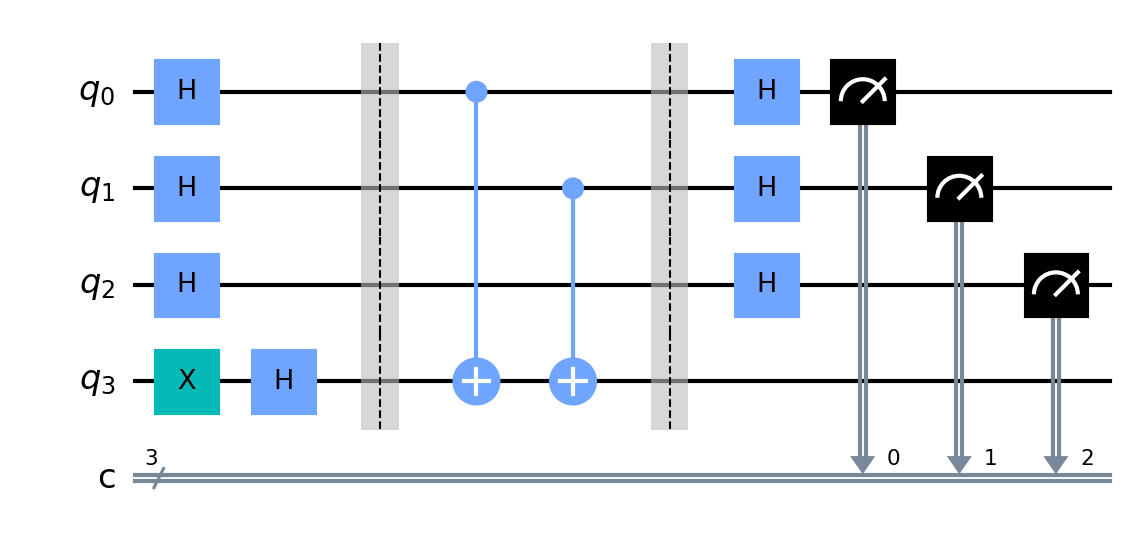
\includegraphics[scale=0.3]{phase_oracle_1.png}
	\captionof{figure}{Exemplo de phase oracle usado para o algoritmo de Deutsch–Jozsa}
	\label{fig:phase-oracle-1}
\end{center}

No exemplo acima, utilizamos o \textit{Phase Kickback} para adicionar uma fase nos qubits 0 e 1, transformando seus estados de $\ket{+}$ para $\ket{-}$, fazendo com que ao serem colapsados o resultado $\ket{1}$ apareça na saída.\\

É possível também criar um phase oracle removendo o qubit adicional (nesse exemplo o Q3), uma vez que podemos utilizar outros gates para introduzir a fase e manter ainda natureza unitária.

\begin{center}
	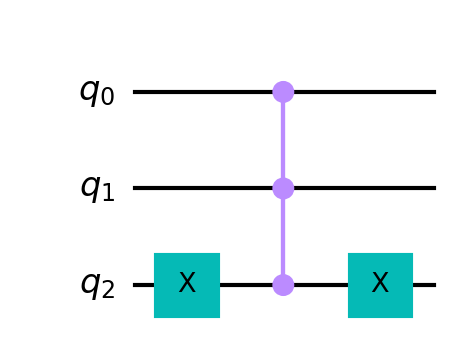
\includegraphics[scale=0.3]{phase_oracle_2.png}
	\captionof{figure}{Exemplo fase Oracle sem a Ancilla}
	\label{fig:phase-oracle-2}
\end{center}


Dessa vez, utilizamos o $MCP$ gate para adicionar uma fase global $\pi$ e dois gates $X$ para dizer quais qubits queremos q tenham o valor 0, codificando assim o valor $011$ ou $3$ na base decimal.

\begin{center}
	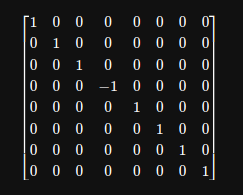
\includegraphics[scale=0.5]{phase_oracle_unitary.png}
	\captionof{figure}{Matriz unitária do Phase oracle}
	\label{fig:phase-oracle-unitary}
\end{center}

É possível verificar então que ao criarmos esse circuito, matemos a matriz identidade e adicionamos a fase $-1$ no valor da coluna relativa ao $011$. \\
Essa versão pode ser considerada como um minimal oracle, uma vez que a própria função interna se mantém unitária, sem a necessidade de ancilla.


\subsection{Boolean Oracle}

O Boolean oracle, por sua vez, representa uma função booleana, sem qualquer adição de fases.\\
Nesse caso, $\ket{x}$ representa a entrada do oracle e $\ket{y}$ represetam os qubits auxiliares que receberam a resposta, $\ket{x}\ket{y} \to \ket{x}\ket{y \oplus f(x)}$.

\subsection{Minimal oracle}

Como já citado anteriormente, o minimal oracle possui uma função que em sua essência é unitária, não requerendo qubits adicionais $\ket{x} \to \ket{f(x)}$.

\begin{center}
	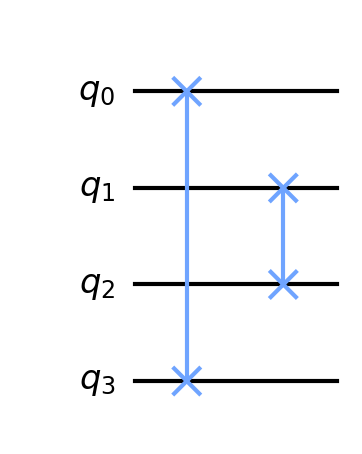
\includegraphics[scale=0.3]{minimal-oracle.png}
	\captionof{figure}{Exemplo de minimal oracle}
	\label{fig:minimal-oracle}
\end{center}

Lembrando que este pode também adicionar fases ao circuito.

\subsection{Simon's Oracle}

O Oracle de Simon, é uma instância do Boolean Oracle. Neste visamos encontrar os períodos da função implementada, ou seja, dado $x$ e $f(x) = y$ existe ao menos uma função em que $f(y) = x$ ?


\begin{center}
	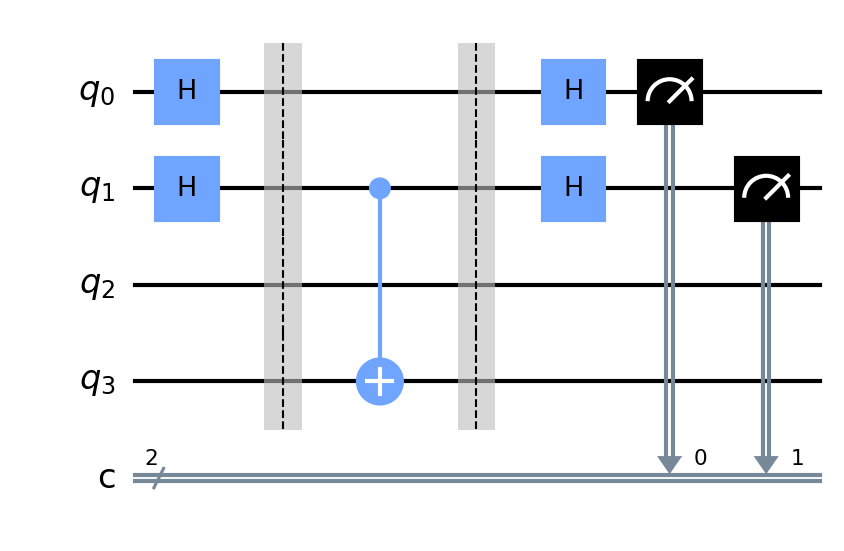
\includegraphics[scale=0.3]{simons.png}
	\captionof{figure}{Exemplo do algoritmo de Simon}
	\label{fig:simons-oracle}
\end{center}

Nesse algoritmo, configuramos uma chave $s$ dentro do oracle, e ao executar o algoritmo temos os possíveis períodos da função, sendo necessário rotinas de pós processamento para identificar o valor correto.

\subsection{QFT(Quantum Fourier Transformation) Oracle}

Por fim, o Oracle QFT aplica a versão quântica da transformada de Fourier, projetando os valores de entrada na base $X$ (também conhecido como base de Fourier).


\begin{center}
	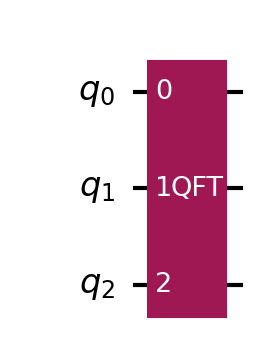
\includegraphics[scale=0.4]{QFT_1.png}
	\captionof{figure}{Exemplo do algoritmo de QFT}
	\label{fig:QFT}
\end{center}

\begin{center}
	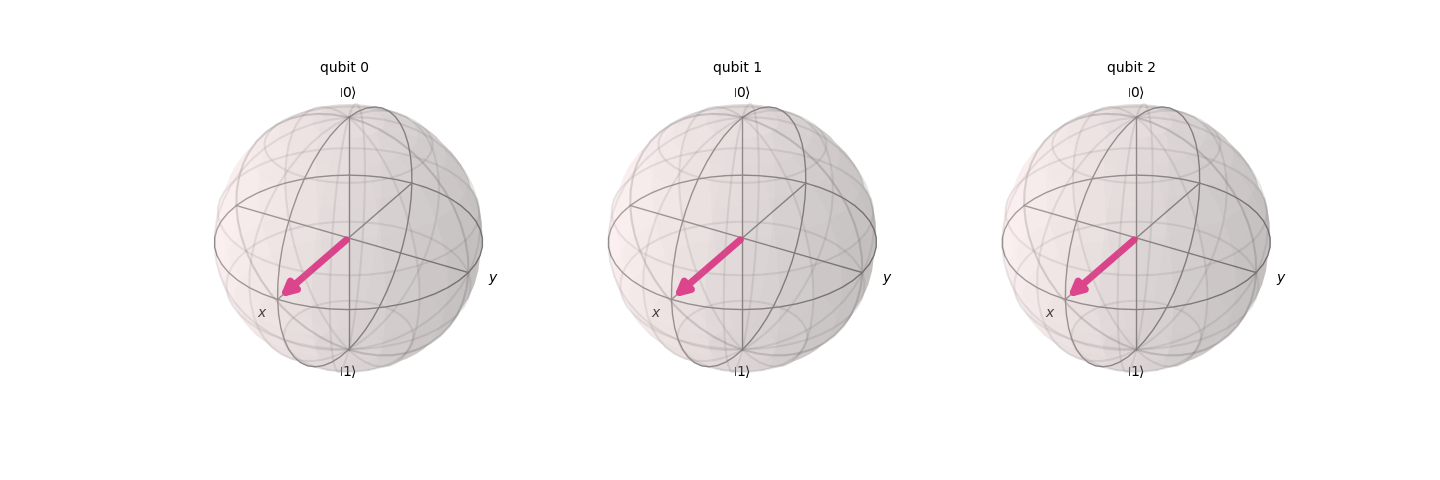
\includegraphics[scale=0.3]{QFT_1_bloch.png}
	\captionof{figure}{Valores mapeados na base de Fourier}
	\label{fig:QFT-bloch}
\end{center}


\section{Desenvolvimento}
\subsection{File Explorer}

Imagine um computador quântico com um sistema operacional quântico (semelhante aos computadores convencionais, mas dessa vez seguindo as leis da mecânica quântica). Pensando nas partes desse sistema operacional, como seria possível pegar arquivos da memória usando a computação quântica?


\subsubsection{Algoritmos usados}

\subsubsection{Grover}
Um dos algoritmos mais comuns para a área é o algoritmo de Grover. Esse algoritmo realiza buscas em "bancos de dados"(bit strings) desorganizados em tempo $O(\sqrt{2^n})$ onde $n$ é o número de qubits usados. Nele, usamos um circuito do qual amplifica-se a probabilidade de encontrar os valores marcados no Oracle na saída.
Tal algoritmo segue o seguinte padrão: \
\begin{enumerate}
	\item{Configuramos todas as possíveis bit strings, ou seja aplicamos uma superposição uniforme $H^{\tens{^n}}$}
	\item{aplicamos o phase oracle $Uf$ do qual implementa uma função que marca os valores que desejamos encontrar}
	\item{aplicamos o operador de Grover Diffuser, $\mathbb{I} - 2 \ket{s}\bra{s}$}, sendo $s$ o estado com o valor que queremos
\end{enumerate}

Convertendo para um circuito temos algo semelhante a:


\begin{center}
	\includegraphics[scale=0.3]{Grover.png}
	\captionof{figure}{Exemplo algoritmo de Grover}
	\label{fig:grover-default-circuit}
\end{center}

Para 1 ou 2 valores, podemos usar a configuração acima. Mas maiores quantidade de valores, precisamos adcionar o conjunto Oracle + Diffuser $k$ vezes, sendo $k \approx { {\pi \over {4 \sqrt{a\over{2^n}}}} - {1\over2}  }$, sendo $a$ o numero de valores marcados.

\subsubsection{Diferença de conjuntos}

Utilizando os phase oracles, podemos criar dois Oracles distintis com ranges de valores diferentes e sobrepor seus valores, realizando a operação de diferença de conjuntos.

\begin{center}
	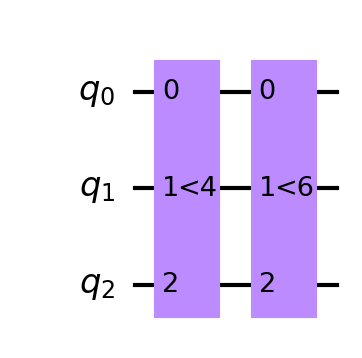
\includegraphics[scale=0.3]{less_than.png}
	\captionof{figure}{Exemplo de diferença de conjuntos}
	\label{fig:less-than-circuit}
\end{center}

Nesse exemplo foi encodado no primeiro oracle o set $\{000, 001, 010, 0110\}$ e no segundo $\{000, 001, 010, 011, 100, 101\}$.

\begin{center}
	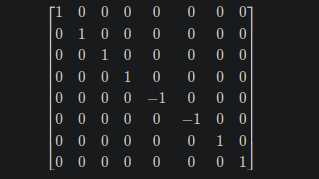
\includegraphics[scale=0.5]{less_than_unitary.png}
	\captionof{figure}{Resultado da diferença de conjuntos}
	\label{fig:less-than-circuit-unitary}
\end{center}

Como pode ser visto, apenas os valores $\{100, 101\}$ permaneceram com a fase, representando então a sobreposição delas.


\subsubsection{Solução para o problema}

Para a solução do problema, podemos criar em uma hash function $C(v)$ da qual recebe o path de um arquivo e retorna uma bit string respectiva. Com essa função em mãos, podemos utilizar o conjunto dos valores retornados e encoda-los em um phase oracle, agindo como uma especie de Look Up Table para os arquivos existentes na máquina.

No entando, para ter sucesso na pesquisa, é necessário utilizar um segundo Oracle encondando $S = P-s$, sendo $s$ o conjunto de arquivos do qual estamos procurando e $S$ os arquivos restantes, aproveitando-se então da diferença de conjuntos para encontrar então apenas os valores desejados para a pesquisa.


\begin{center}
	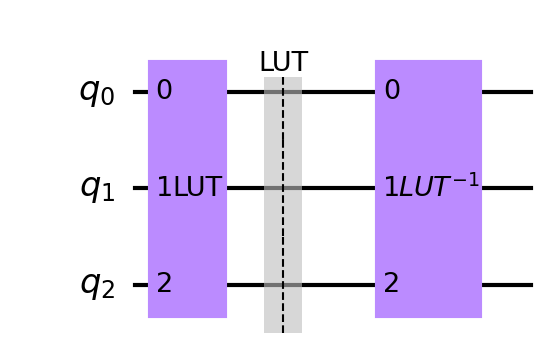
\includegraphics[scale=0.6]{sets-difference-look-up-table-oracle.png}
	\captionof{figure}{Diferença de conjuntos com as Look Up Tables}
	\label{fig:luts}
\end{center}

Sendo assim, o primeiro oracle age como o HD da marquina, marcando todos os arquivos existentes, e o segundo age como o mediador da pesquisa.

Com isso, adicionamos a Look Up Table final ao algoritmo de Grover.

\begin{center}
	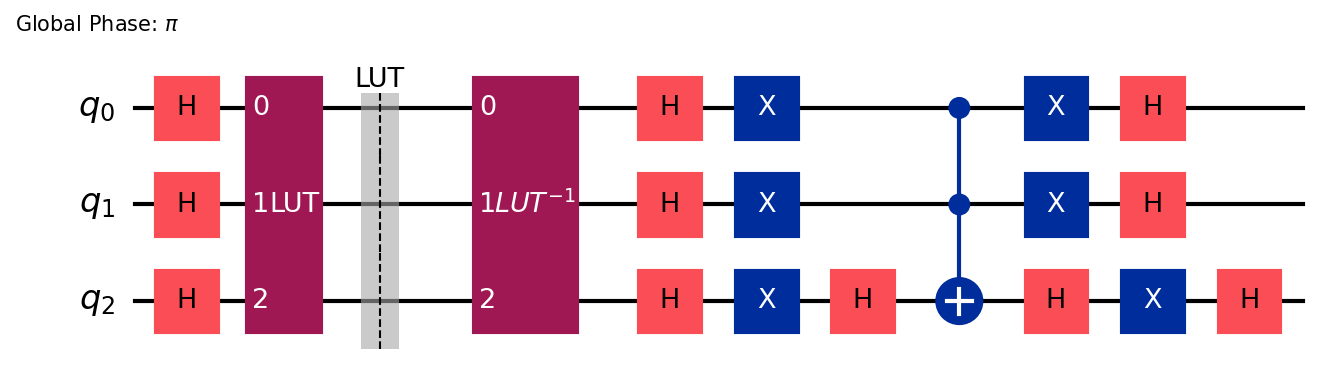
\includegraphics[scale=0.5]{file_explorer.png}
	\captionof{figure}{File explorer circuito}
	\label{fig:file-explorer}
\end{center}

\subsubsection{Resultados}

Para um caso hipotetico de sistema completamente quântico, certamente esse é um das maneiras de encontrar arquivos em meio a todos os outros.

Contudo, como o objetivo dessa pesquisa sugere, para utilizar esse modelo em um sistema clássico tomando proveito da computação quântica, não se mostra como a melhor opção.

Para sistemas convencionais, dos quais utilizam métodos baseados em árvores, não é possivel tirar qualquer proveito aqui, sendo $O$ polinomial contra $O$ quadrático.

Mesmo perante os testes clássicos feitos durante o desenvolvimento, esse protocolo só se mantém util quando a pesquisa era feita de forma linear.


\begin{center}
	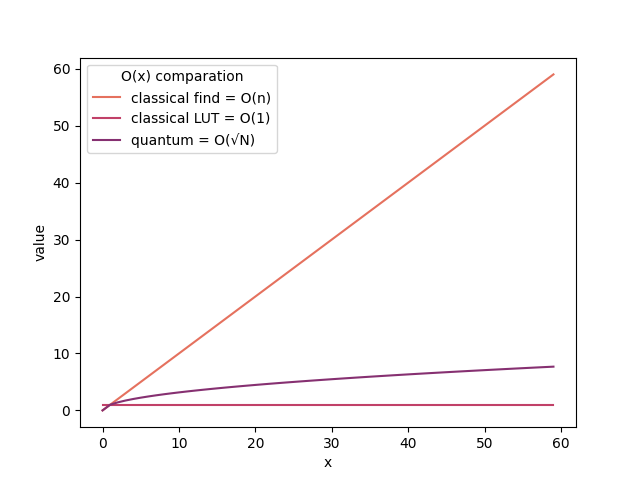
\includegraphics[scale=0.5]{algorithms-finding-comparation.png}
	\captionof{figure}{Comparação algoritmos usados na pesquisa}
	\label{fig:file-explorer-comparation-O}
\end{center}

Sendo assim, o algoritmo de Grover deve ser pensando para casos do qual a versão clássica possui complexidade $\ge O(n)$.


\subsection{Milhas para quilômetros}

O segundo problema testado foi a conversão de milhas para Km. Essa idéia se deu a após a descoberta de um algoritmo capaz de calcular fibonacci com circuitos quânticos.

\subsubsection{algoritmo de Fibonacci}

A versão quântica usada para calcular fibonacci apresentada em \cite{gilliam2020canonical}, demonstra que utilizando um circuito que coloca em superposição todas as bit strings com $n$ qubits que não possuem valores uns consecutivos, é possivel encontrar o valor $n$ de fibonacci.

Sua implementação se dá da seguinte maneira:

\begin{center}
	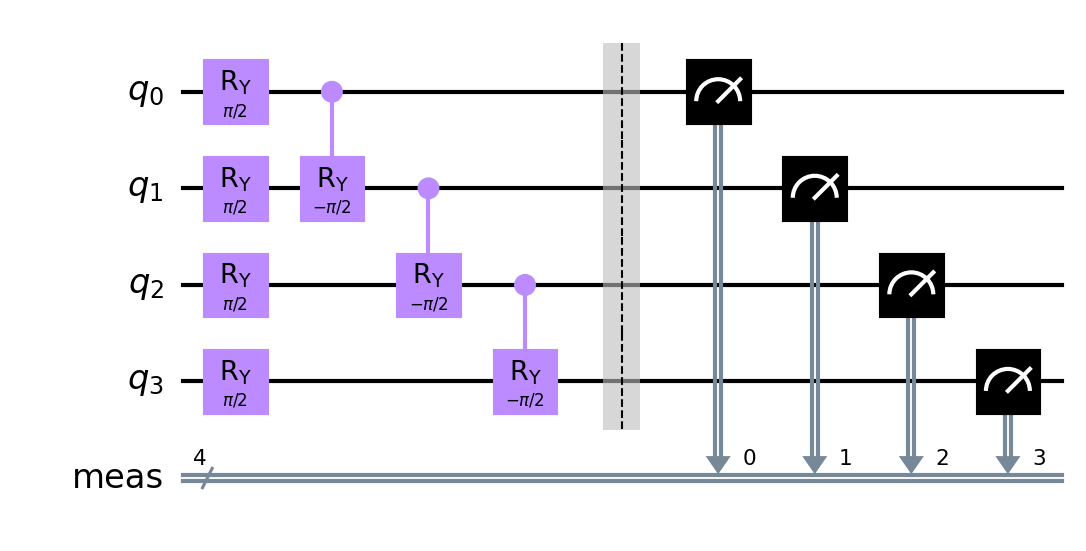
\includegraphics[scale=0.3]{fibonacci-circuit.png}
	\captionof{figure}{Exemplo Algoritmo de Fibonacci}
	\label{fig:fibonacci-circuit}
\end{center}

Tendo como resultado:

\begin{center}
	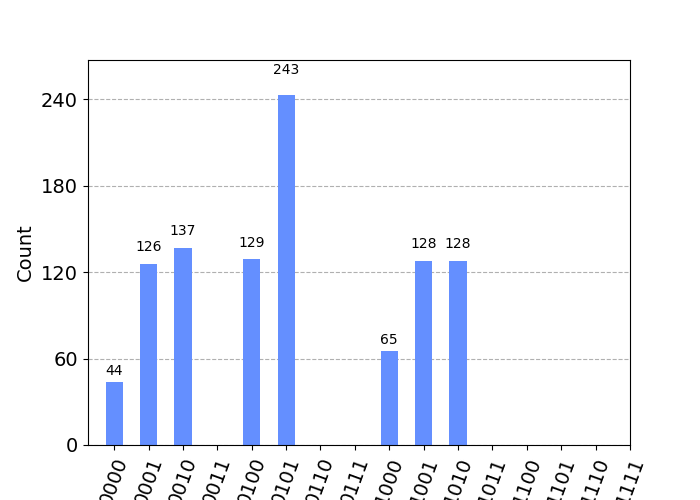
\includegraphics[scale=0.5]{fibonacci-4.png}
	\captionof{figure}{Resultado exemplo Fibonacci - F(4)}
	\label{fig:fibonacci-circuit-result}
\end{center}

Essa implementação inicia a cadeia partir do valor $2$, sendo assim: $2, 3, 5, 8, 13, 21, ...$. 
Repare que na figura \ref{fig:fibonacci-circuit-result}, a quantidade de número de valores encontrados (nesse caso $8$) é o mesmo do que o 4º valor da sequência. Ou seja, para esse circuito, o valor de qubits $n$ representa o valor $n$ de fibonacci que queremos encontrar. Sendo assim, podemos pensar em um oracle implementado $F(n)$ do qual a entrada $n$ é igual a $\ket{0}^{\tens^n}$.

\subsubsection{Implementação}

Para aproximar o valor de milhas para quilômetros, podemos utilizar a relação de fibonacci da seguinte forma:

$F_{km} = F_{milhas}(n+1)$, sendo assim, para conseguir o valor relativo em quilômetros, basta pegar o próximo valor na sequência.


\begin{table}[!h]
	\begin{center}
		\begin{tabular}{ |c|c| } 
			\hline
			milhas & km \\
			\hline
			1 & 2 \\
			\hline
			2 & 3 \\
			\hline
			3 & 5 \\
			\hline
			5 & 8 \\
			\hline
		\end{tabular}
	\caption{valores aproximados de milhas para Km}
	\end{center}
\end{table}

No entanto, dessa forma, temos um problema, a quantidade necessária de qubits. Para entradas $n$ tendendo ao infinito, precisaremos de infinitos qubits. Para resolver isso, foi criado um algoritmo clássico simples para quebrar numero desejado em partes menores que podem ser calculadas em um circuito com menos qubits, $ f: (n) \to ((n_1, i), (n_2, i), ...)$, mapeando então a entrada $n$ para uma lista de tuplas contendo o número base e a quantidade de aplicações necessária $i$.

Com isso, o circuito final é apresentado da seguinte forma:

\begin{algorithm}
	\begin{algorithmic}
		\For{cada número base n}
		
			Aplique o oracle F(n)
			
			Faça as medições nos qubits
			
			reset os qubits usados
			
		\EndFor\\
		
		verifique o resultado de cada bit string\\
		
		multplique cada resultado com o valor i correspondente
		
	\end{algorithmic}
	\caption{Algoritmo quântico para a conversão}
	\label{alg:miles-to-km-quantum-algortihm}
\end{algorithm}

\begin{center}
	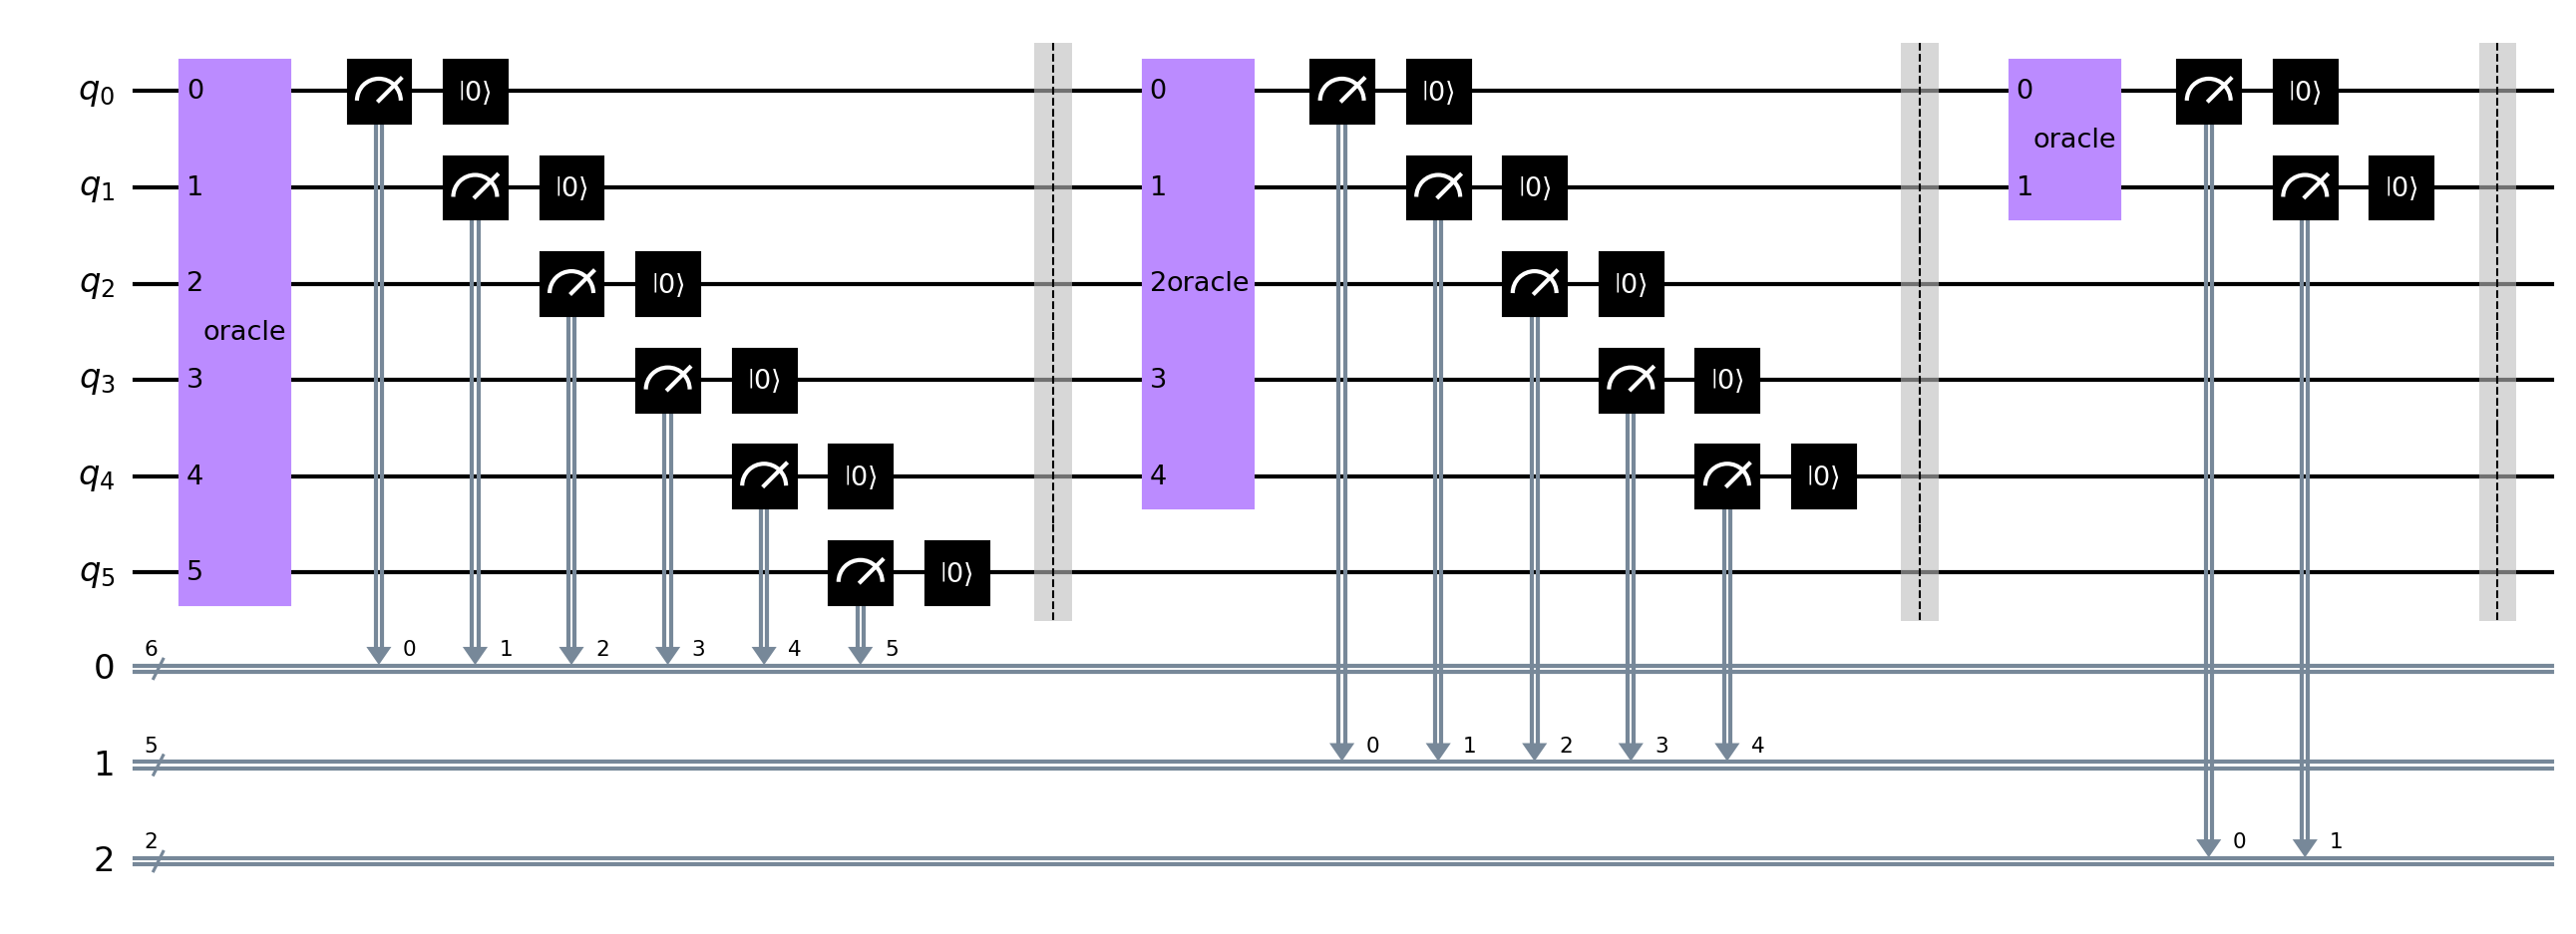
\includegraphics[scale=0.15]{number_breakdown_circuit.png}
	\captionof{figure}{Circuito de conversão implementado}
	\label{fig:miles-km-circuit}
\end{center}

\subsubsection{Resultados}

Usando esse método é possível alcançar os valores esperados. Contudo existem alguns pontos que torna esse método pior do que a versão clássica:

\begin{enumerate}
\item{Quantidade necessária de mediçoes e tempo de execução}\\
Para cada vez que medirmos o circuito, precisamos de uma quantidade alta de shots para alcançar um resultado melhor, aumentando também o tempo necessário para executar desse versão.

\begin{center}
	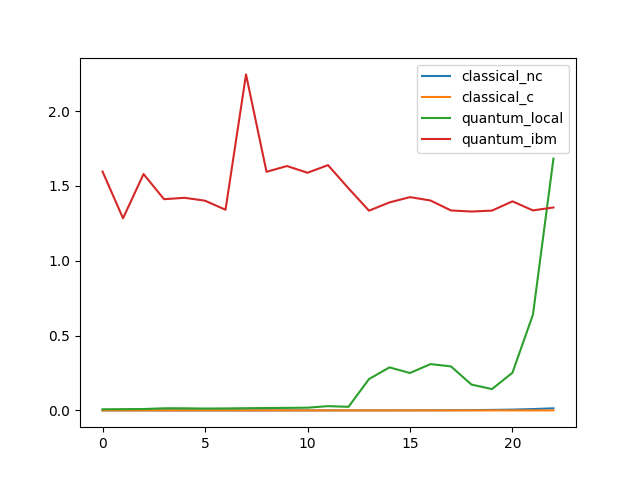
\includegraphics[scale=0.6]{comparison_miles_to_km.png}
	\captionof{figure}{Comparação tempos de execução}
	\label{fig:comparasion-miles-km-time}
\end{center}

Como é possivel ver em \ref{fig:comparasion-miles-km-time}, o tempo das versões clássicas com e sem memoization possuem tempo praticamente constante de execução em comparação com as versões quânticas em simuladores e hardwares reais.


\item{Erros}\\
Como a maioria dos algoritmos quanticos da era NISQ(noisy intermediate-scale quantum), os erros também estão presentes, e por utilizarmos muitos gates de dois qubits, esses erros podem se intensificar dependendo do hardware usado.

\item{Imprecisão conforme a entrada cresce ao infinito}\\

\begin{center}
	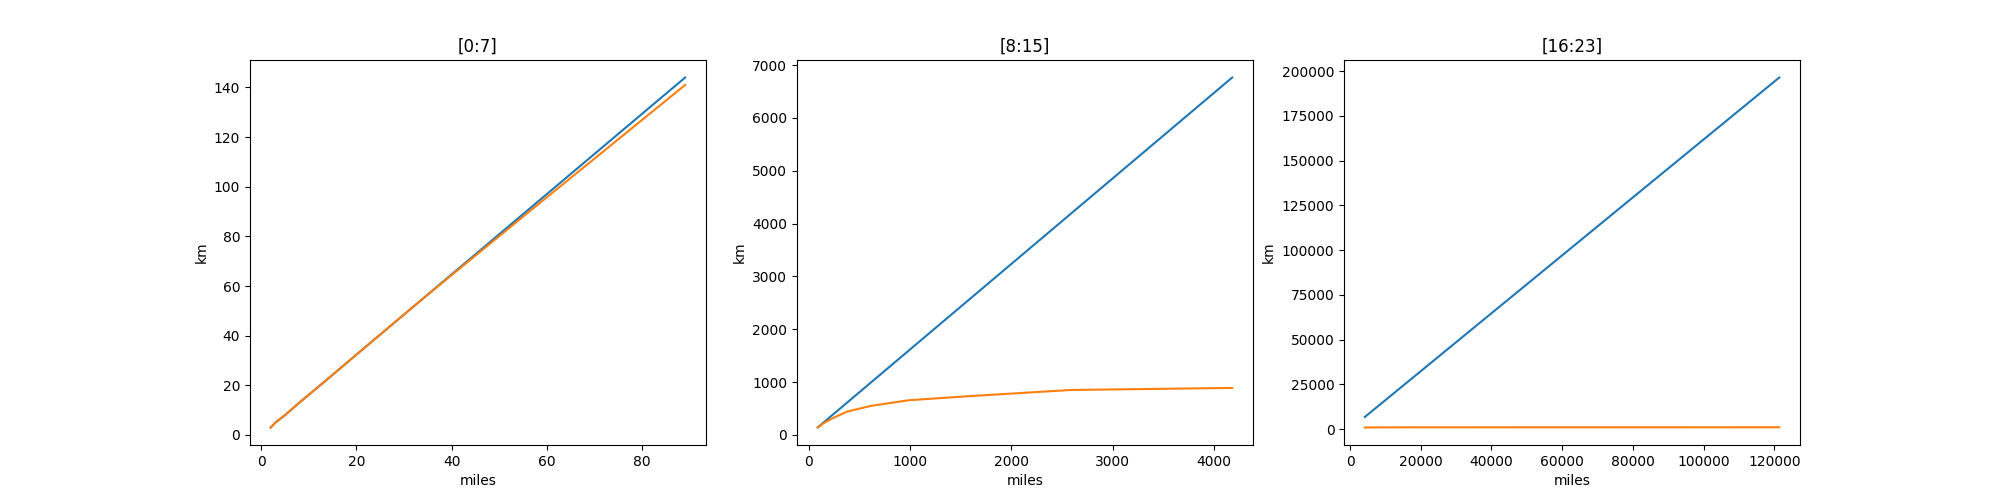
\includegraphics[scale=0.2]{miles_to_km_defiance.png}
	\captionof{figure}{Comparação resultados versão clássica e quântica}
	\label{fig:values-miles-km-quantum}
\end{center}

Como é possível ver em \ref{fig:values-miles-km-quantum}, valores pequenos possuem uma boa precisão com os números esperados(em azul), mas apartir de certo ponto eles começam a se distanciar.


\item{necessidade de intervenção clássica}

Por fim, esse algoritmo requer que seja primeiro verificado quais são os valores de fibonacci necessários para cada parte, além de ser necessário pós processamento após as medições.

Para amenizar tal problema, é necessário criar outros algoritmos capazes de encodar o valor requerdio diretamente no circuito sem maiores intervenções clásssicas, necessitando apenas de pós processamento (em certos casos).

\end{enumerate}

\subsection{Torres de Hanoi Hanoi}

Para o terceiro teste, foi implementado uma versão das torres de Hanoi usando os Oracles como meio de encoding.

\subsubsection{Implementação}

Para implementar as torres de hanoi em um oracle, são necessários $(\floor{\log_2{x}}} + 1) * 3$ qubits, sendo $x$ o número de discos com a seguinte ordem $\ket{t_{n-1} t_{n-2} ... t_0}\ket{a_{n-1} a_{n-2} ... a_0}\ket{s_{n-1} s_{n-2} ... s_0}$, sendo $t$ a ultima torre, $a$ a torre do meio e $s$ a primeira torre, e $n = {{n \space qubits} \over 3}$.

Com essa configuração, os numeros de $1$ à $x$ são codificados em um phase oracle, e em seguida são realizadas operaçoes de $swap$ para modificar a posição dos valores binários e mover os valores do $n$ qubits menos significativos, para os $n$ qubits mais significativos.

\begin{center}
	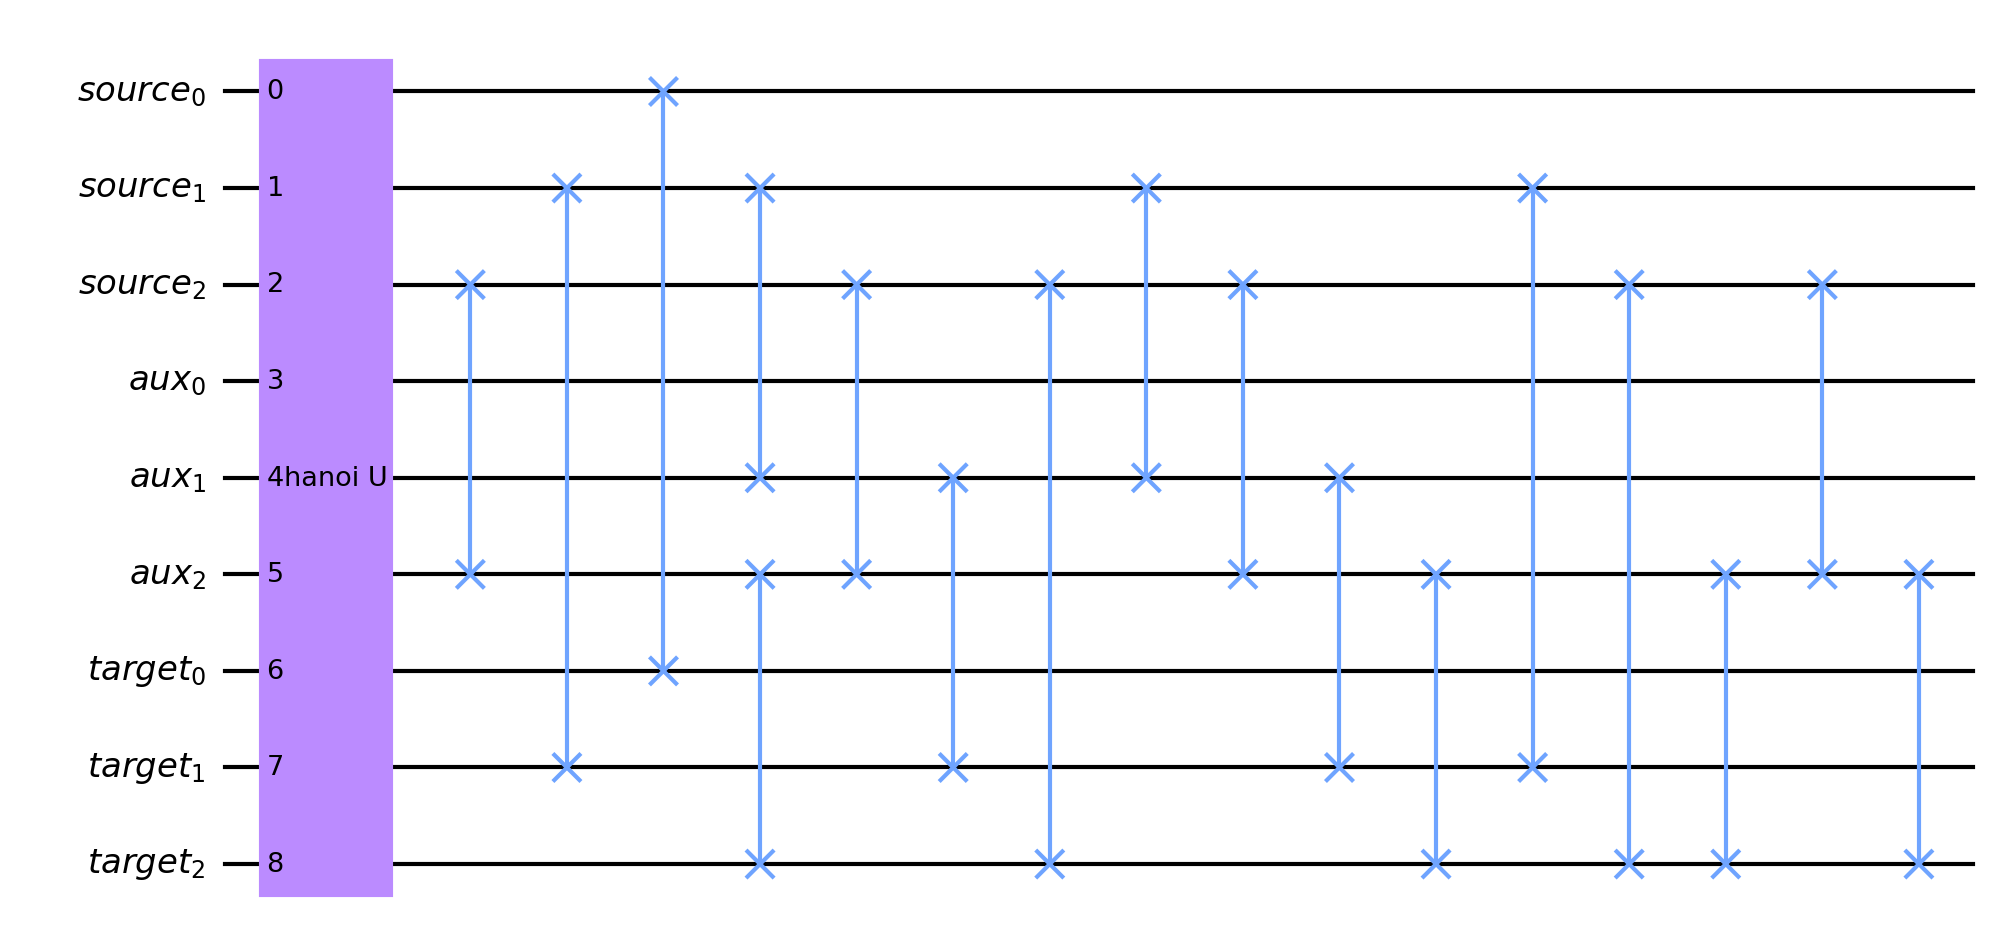
\includegraphics[scale=0.2]{hanoi_4_discs.png}
	\captionof{figure}{Torre de hanoi com 4 discos}
	\label{fig:hanoi}
\end{center}

Nesse formato, é possível utilizar o unitário gerado pelo oracle, assim como o algoritmo de Grover para verificar o resultado.

\subsubsection{Resultados}

Nessa implementação, o algoritmo segue o mesmo padrão da versão clássica, sendo o melhor ou pior desempenho dependendo estritamente do hardware usado.


\subsection{Buckshot Roulette}

Buckshot Roulette é um jogo feito pelo desenvolvedor \href{https://mikeklubnika.itch.io/}{Mike Klubnika} para computador que toma como base a premissa de reinventar a infame roleta russa. No jogo, você é desafiado por um demônio (dealer), e caso você ganhe você ganha uma recompensa, mas caso contrário o jogo reinicia.

Para esse projeto, tomamos como base a primeira rodada do jogo buscando encontrar a melhor estrategia para maximizar os ganhos.

Nessa primeira rodada temos 3 vidas, 2 balas falsas e 1 bala verdadeira.

A dinamica funciona da seguinte forma: você começa jogando,tendo duas possíveis escolhas, atirar em você mesmo ou no dealer. Caso você atire em você mesmo e a bala for real, você perde uma vida, mas você joga novamente na próxima rodada, caso a bala seja falsa você joga novamente. Agora, caso a escolha seja atirar no dealer, se a bala for real você ganha, se não o dealer joga.


\subsubsection{Versão clássica}

Antes de crair o circuito, foi feita a modelagem do jogo usando a estrutura em árvore.

\begin{center}
	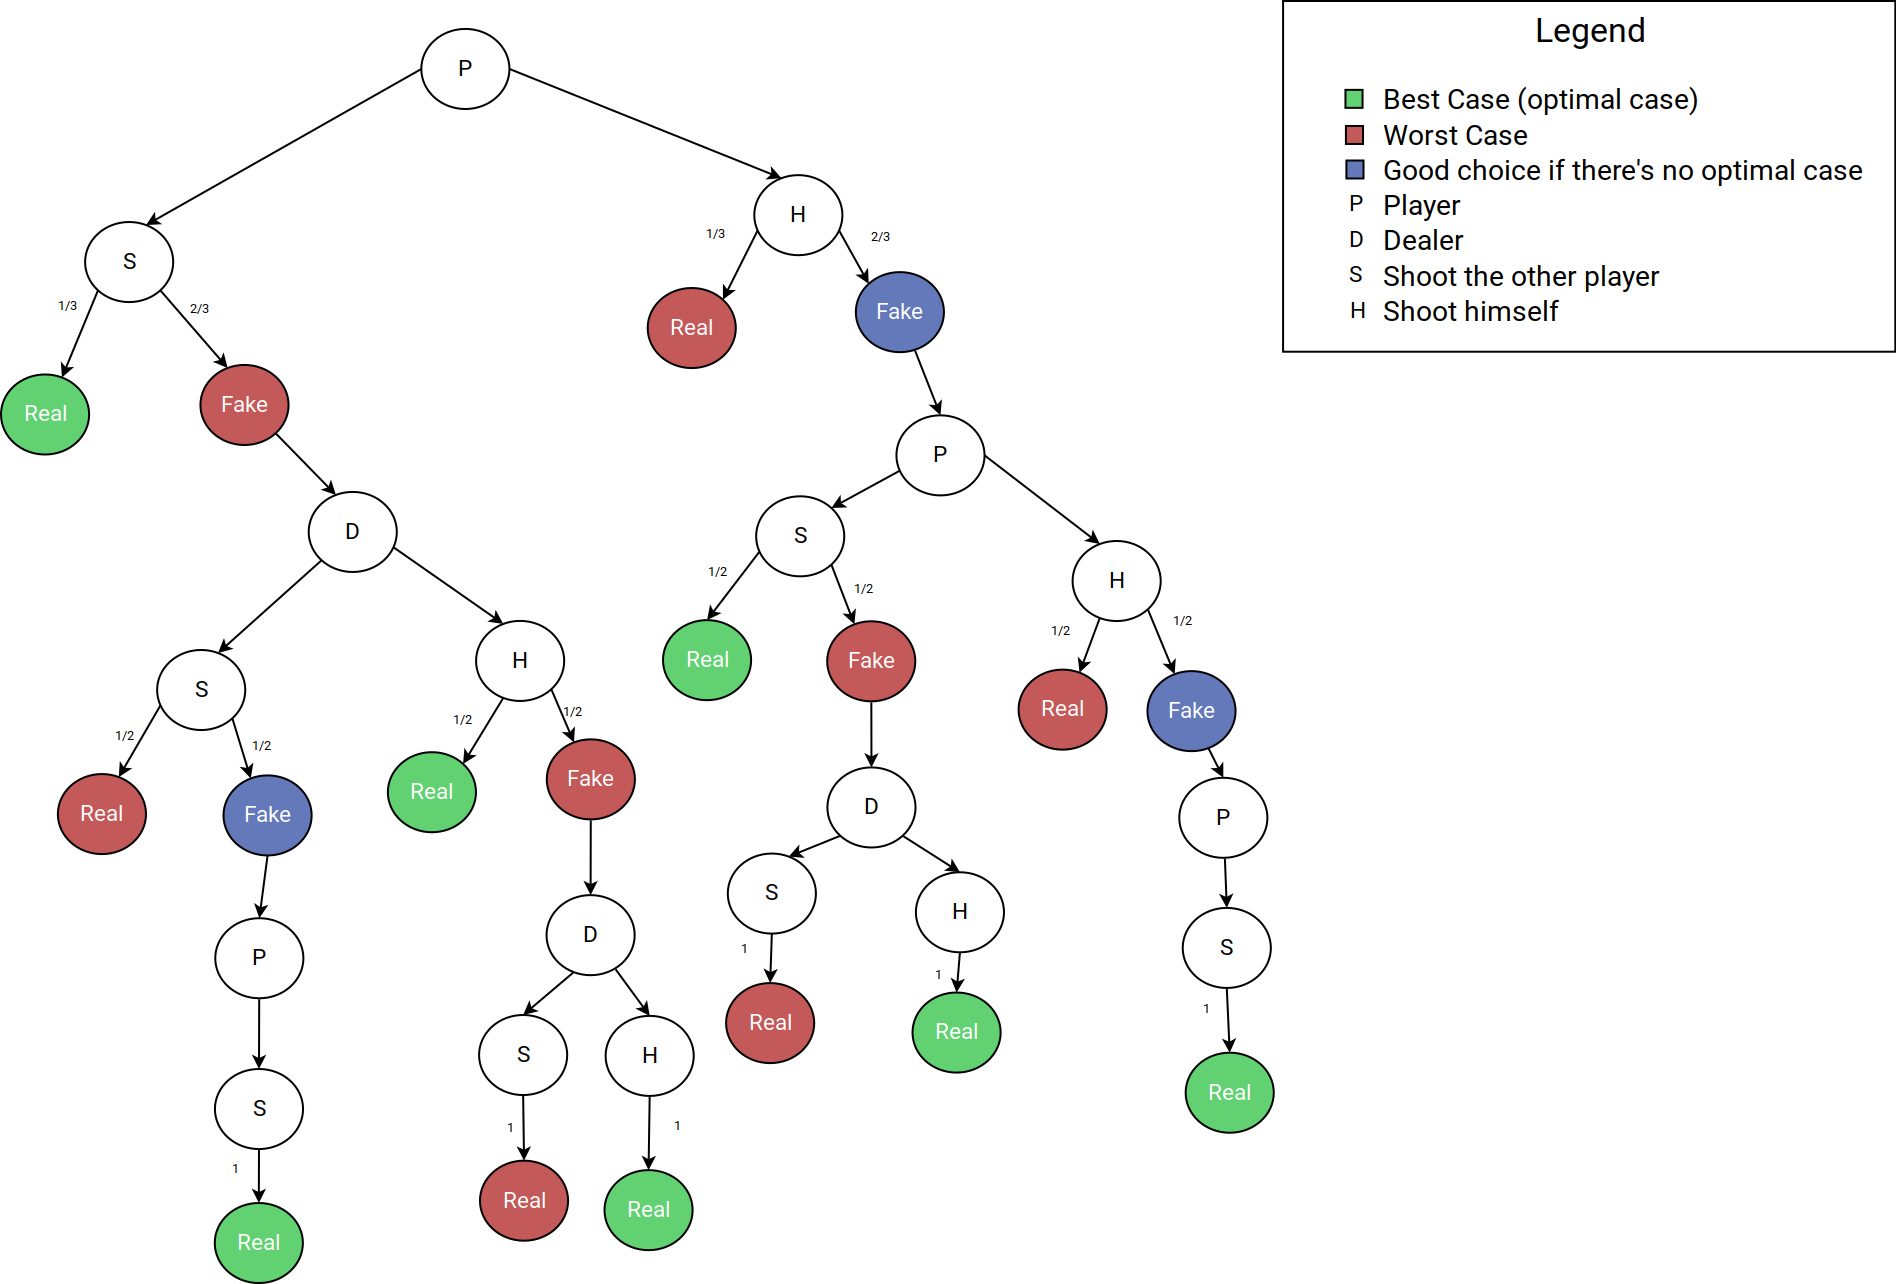
\includegraphics[scale=0.2]{buckshot-roulette-diagram.png}
	\captionof{figure}{Buckshot Roulette diagrama}
	\label{fig:classical-model-bckr}
\end{center}

Note que nessa estrutura, o dealer na ultima bala, ainda pode escolher atirar ou não nele mesmo, isso acontence pois o jogo implementa ações randomicas para o dealer.

Seguindo essa estrutura, podemos tentar encontrar o melhor caminho dentre a àrvore e simular os resultados da partida.


\begin{center}
	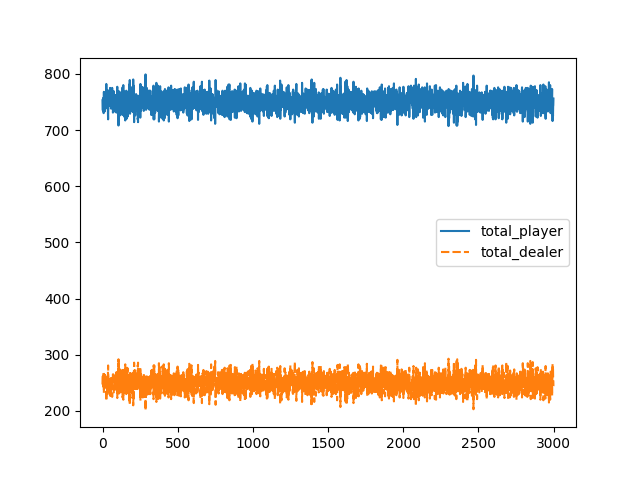
\includegraphics[scale=0.6]{optimal_player_strategy.png}
	\captionof{figure}{Buckshot Roulette clássico - melhor estratégia}
	\label{fig:classical-model-bckr-optimal-strategy}
\end{center}

Após testar os possíveis caminhso, o melhor resultado obtido foi esse apresentado acima em \ref{fig:classical-model-bckr-optimal-strategy}. Com um pouco de investigação, foi possível entender que a melhor estratégia encontrada foi o player começar atirando no dealer. Isso pois ao seguir tal caminho, ele tem uma chance a menos de perder a rodada, já que a chance de perder logo no começo é eliminada.




\begin{table}[!h]
	\begin{center}
		\begin{tabular}{ |c|c|c|c| } 
			\hline
			rodada & ação & resultado da ação & resultado da partida \\
			\hline
			1 & player atira no dealer  & real & player ganha\\
			\hline
			1 & player atira no dealer  & fake & -\\
			\hline
			2 & dealer atira no player  & real & dealer ganha\\
			\hline
			2 & dealer atira no player  & fake & -\\
			\hline
			2 & dealer atira nele mesmo  & real & player ganha\\
			\hline
			2 & dealer atira nele mesmo  & fake & -\\
			\hline
			3 & player atira no dealer  & real & player ganha\\
			\hline
			3 & dealer atira no player & real & dealer ganha\\
			\hline
			3 & dealer atira nele mesmo  & real & player ganha\\
			\hline
		\end{tabular}
		\caption{melhor estratégia - possíveis resultados}
	\end{center}
\end{table}

\subsubsection{Versão quântica}

A partir dessa ideia, um circuito quântico foi modelado imitando o primeiro round, e um oracle foi usado para cada jogador implementando sua estratégia em seu interior.

\begin{center}
	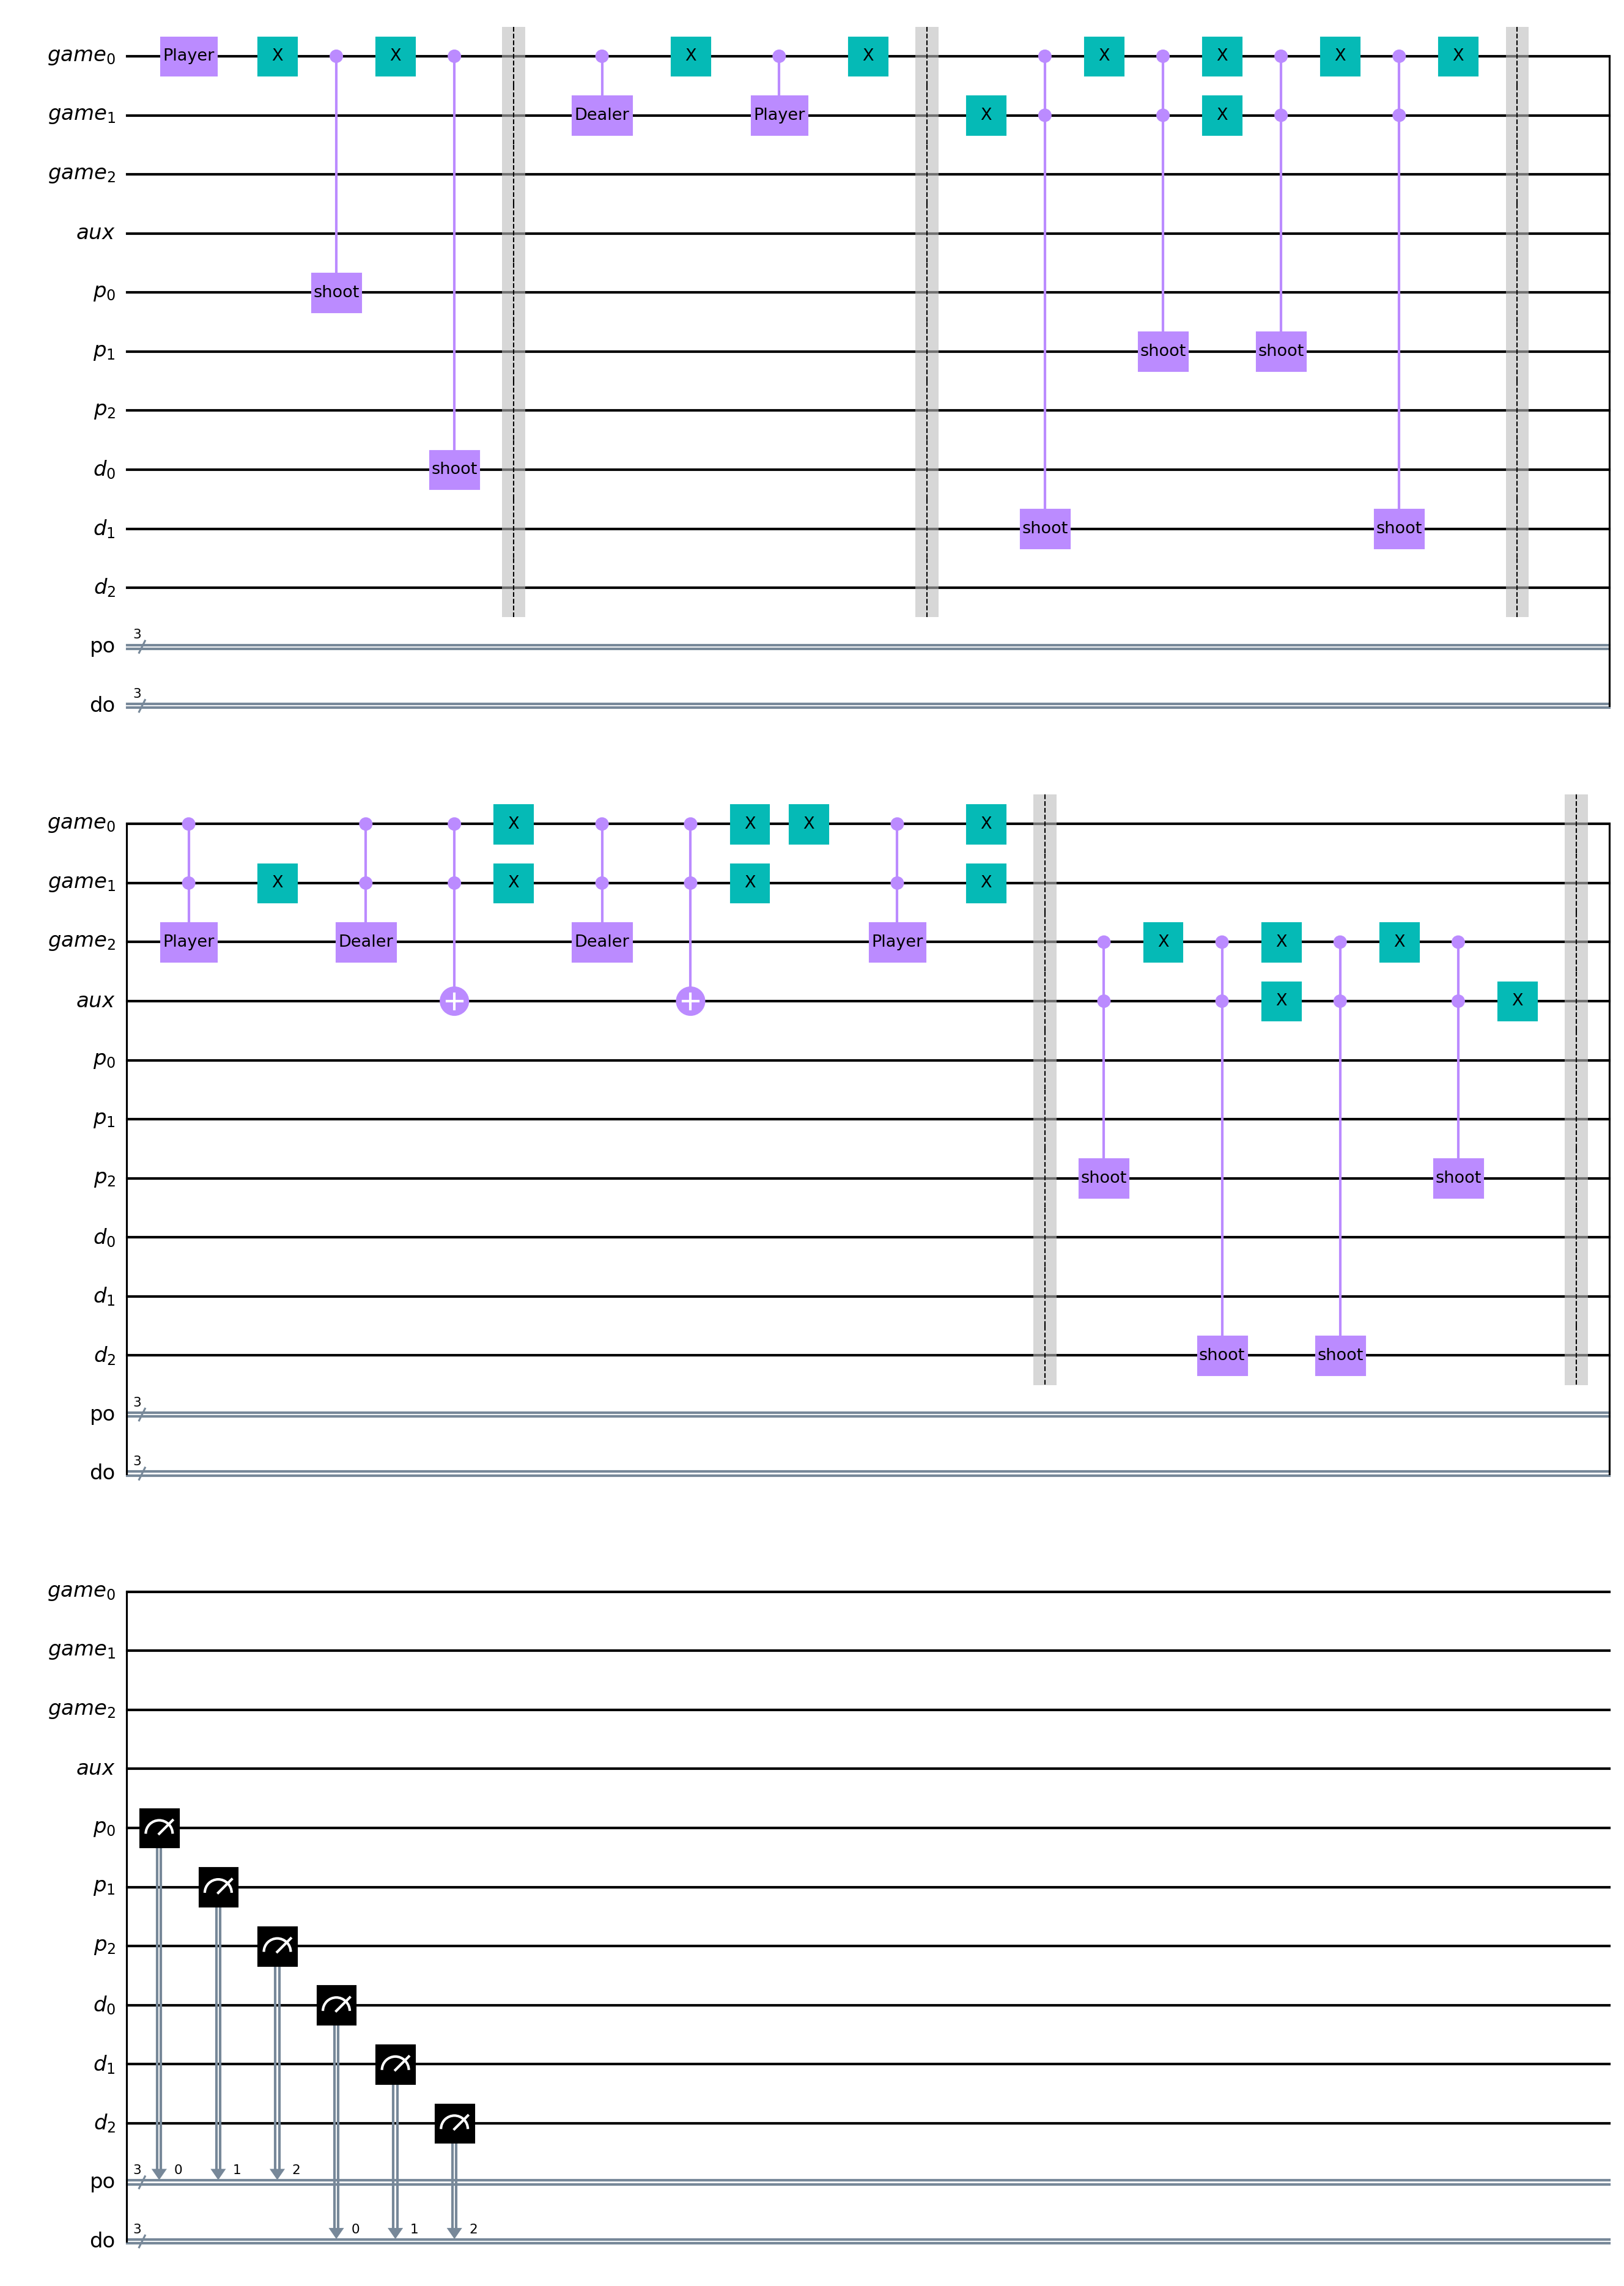
\includegraphics[scale=0.3]{quantum_buckshot_roulette.png}
	\captionof{figure}{Circuito para o buckshot roulette}
	\label{fig:bckr-circuit}
\end{center}

Além disso, para encontrarmos a melhor estratégia para o player, foi inserido dois parâmetros dentro do oracle, sendo possível inserir qualquer valor $\theta$ e $\phi$ para encontrar a melhor rotação na bloch sphere. 

Após verificar uma grande variedade de valores possíveis, a rotação que entregou o melhor resultado foi $\theta = 3.0853981633974477, \phi=5.685398163397447$.
Usando essa estratégia, os resultados foram semelhantes a versão clássica usando o simulador Aer:

\begin{center}
	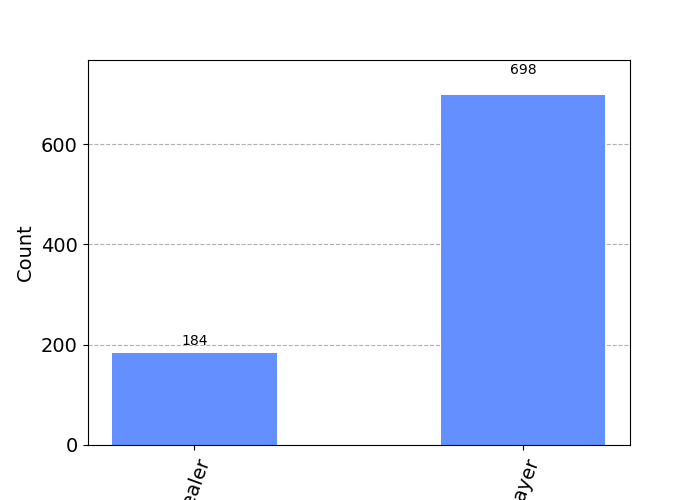
\includegraphics[scale=0.6]{final_buckshot_roulette_quantum_optimal_strategy.png}
	\captionof{figure}{Resultado Buckshot Roulette quântico}
	\label{fig:bckr-circuit-result}
\end{center}

Observando a bloch sphere do estado gerado por essa rotação, é possível ver também que a estratégia de fato se assemelha a versão classica, com o player preferindo atirar no dealer a maior parte do tempo (o valor 1 aqui representa atirar no outro jogador e 0 atirar em si mesmo).

\begin{center}
	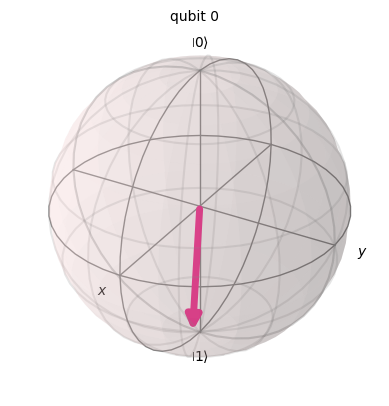
\includegraphics[scale=0.6]{player_optimal_strategy_bloch.png}
	\captionof{figure}{Melhor estratégia Buckshot Roulette quântico - Bloch Sphere}
	\label{fig:bckr-bloch-sphere-best-strategy}
\end{center}

\subsubsection{Conclusões}

Para esse problema, não há uma competição certa entre as duas versões, uma vez que uma é diretamente inspirada na outra.

Além disso, a versão quântica possui ainda a possibilidade de explorar mais valores do que a versão clássica, deixando o player mais aberto a escolha de estratégias.

Em relação a erros providos pelo hardware não afeta diretamente os resultados, uma vez que mesmo com os erros a proporção se mantém.


 \begin{center}
 	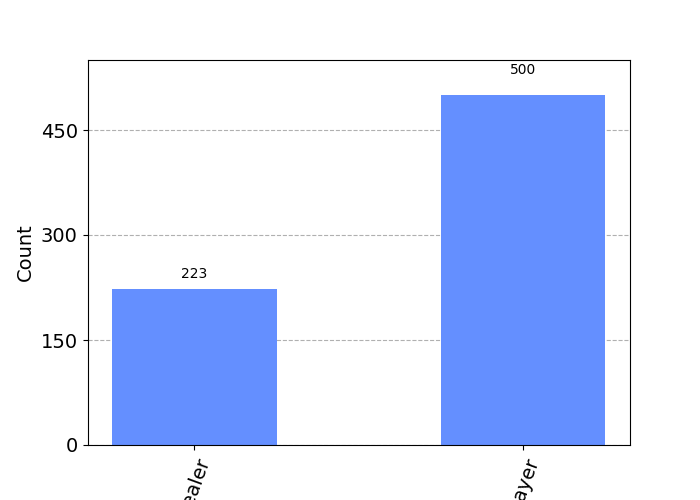
\includegraphics[scale=0.6]{final_buckshot_roulette_quantum_optimal_strategy_fake_melbourne.png}
 	\captionof{figure}{Resultados Buckshot Roulette usando o fake backend Melbourne da IBM}
 	\label{fig:bckr-fake-melbourne}
 \end{center}

Note também que o total de partidas ganhas não chega ao total jogado, 1000 partidas no total, isso pois, pelo design do circuito, não é possível verificar a jogada do player anterior, sendo possível continuar jogando mesmo que um dos players já tenham perdido, o que foi necessário correções usando pós processamento após a simulação.

Em suma, ambos as simulações atingiram o mesmo resultado e foi demonstrado que é possível usar aqui o quantum oracle como uma representação de um player dentro do circuito.

\subsection{QRAM}
Por fim, o último projeto realizado foi o de uma QRAM utilizando os oracles para encodar os valores desejados. Nessa versão, foi testado maneiras de criar QROMs (com dados estaticos dentro), e uma possível maneira de utilizar uma QRAM habil para escrita.

Neste, foi levado em consideração o armazenamento de estados quânticos, e não de bitstrings clássicas.

\subsubsection{QROM}

Primeiro, foi feita uma versão de QROM, do qual utiliza $n$ qubits para endereços e $m$ qubits para a criação dos estados. Não necessáriamente os valores precisam estar correlacionados, podemos ter $n=3, m=10$. Isso pois, nesse formato, podemos mapear diversas superposições diferentes e aplicálas quando certo endereço for chamado. Sendo assim, o algoritmo aqui mostrado armazena os valores a partir da configuração de gates controlados interiores ao oracle, criando uma superposição apenas quando certo valor de entrada é inserido.

A entrada do circuito segue o seguinte formato: ${\ket{0}^{\tens^m}} {\ket{a_{n-1} a_{n-2} ... a_0}}$


\begin{center}
\end{center}

\nocite{SOARE2009368}
\nocite{odonnell_2015_lecture}
\nocite{bacon_2006_cse}
\nocite{lipics_stacs}
\nocite{odonnell_2015_lecture_2}
\nocite{brodkorb_2019_the}
\nocite{amreen_oracle}
\nocite{kalyanasyndaram_2021_mod04lec23}
\nocite{davis_2006_turing}
\nocite{viswanathan_2013_reductions}
\nocite{Fan_2007}
\nocite{cryptoeprint:2020/1270}
\nocite{buhrman1998quantum}
\nocite{sanchezrivero2023initial}
\nocite{gilliam2020canonical}
\nocite{Kashefi_2002}
\nocite{e21080800}
\nocite{Zeng_2014}
\nocite{atici2004comparative}
\nocite{sundarappan_2022_how}
\nocite{dai_view}
\nocite{sep-game-theory}
\nocite{Giovannetti_2008}
\nocite{jaques2023qram}
\nocite{PythonEWL2022}
\nocite{frackiewicz2011application}
\nocite{Eisert_1999}
\nocite{usman_2019_kilometres}
\nocite{ldiaandr_2021_tower}
\nocite{diptokarmakar47_2019_how}
\nocite{a2020_towers}
\nocite{geeksforgeeks_2014_program}
\nocite{khan_2021_quantum}
\nocite{legn_2022_dilemma}
\nocite{siegelwax_2022_quantum}
\nocite{landi_density}
\nocite{bacon_2006_cse}
\nocite{vijayakrishnan_2019_role}
\nocite{python_scientific}
\nocite{scipyoptimizeminimize_scalar}
\nocite{davis_optimization}
\nocite{scipyoptimizeminimize}



\bibliographystyle{unsrt}
\bibliography{references}


\end{document}
